%% The following is a directive for TeXShop to indicate the main file
%%!TEX root =../diss.tex

\chapter{Future Work}
\label{ch:futurework}

\section{Exploring the link between perfusion and oxygenation}

\subsection{Comparing DCE-MRI perfusion patterns with \ac{dOE-MRI} oxygenation patterns}

One SCCVII and one HCT-116 tumour-bearing mouse were catheterized and injected with 30mM solution of Gd-DTPA for DCE-MRI at a rate of 1mL/min using a power injector at a dose of 5$\mu$L/g.

\noindent\textbf{Perfusion maps:} Signal intensity timecourse from the DCE-MRI map was first normalized to the mean signal intensity pre-injection.
Area under the first 60 seconds of the normalized signal intensity enhancement curve after the injection was calculated (\acs{AUC}$_{60}$) using the composite Simpson's Rule (\texttt{scipy.integrate.simps}).
A binary ground-truth perfusion map was constructed by classifying all voxels with IAUC$_{60} > 0$ as perfused and everything else as unperfused.

Where \ac{dOE-MRI} and DCE-MRI scans were acquired in the same SCCVII and HCT-116 tumour-bearing mice,  maps of oxygenation status were compared to IAUC$_{60}$ perfusion maps, as shown in Figure~\ref{fig_perfusion}.
Mean IAUC$_{60}$ for the well-perfused SCCVII tumour was 22 $\pm$ 16 \%$\cdot$s and for the comparatively poorly perfused HCT-116 tumour was 7$\pm$ 7 \%$\cdot$s.
Well-oxygenated O$_2$-positive regions generally correspond to perfused, high IAUC$_{60}$ areas in both SCCVII and HCT-116 tumours.
A large patch of necrosis, as identified in histological section, in the HCT-116 tumour was also extremely poorly perfused; such large patches of necrosis were not present in the SCCVII tumour.

\begin{figure}[htbp]
   \centering
   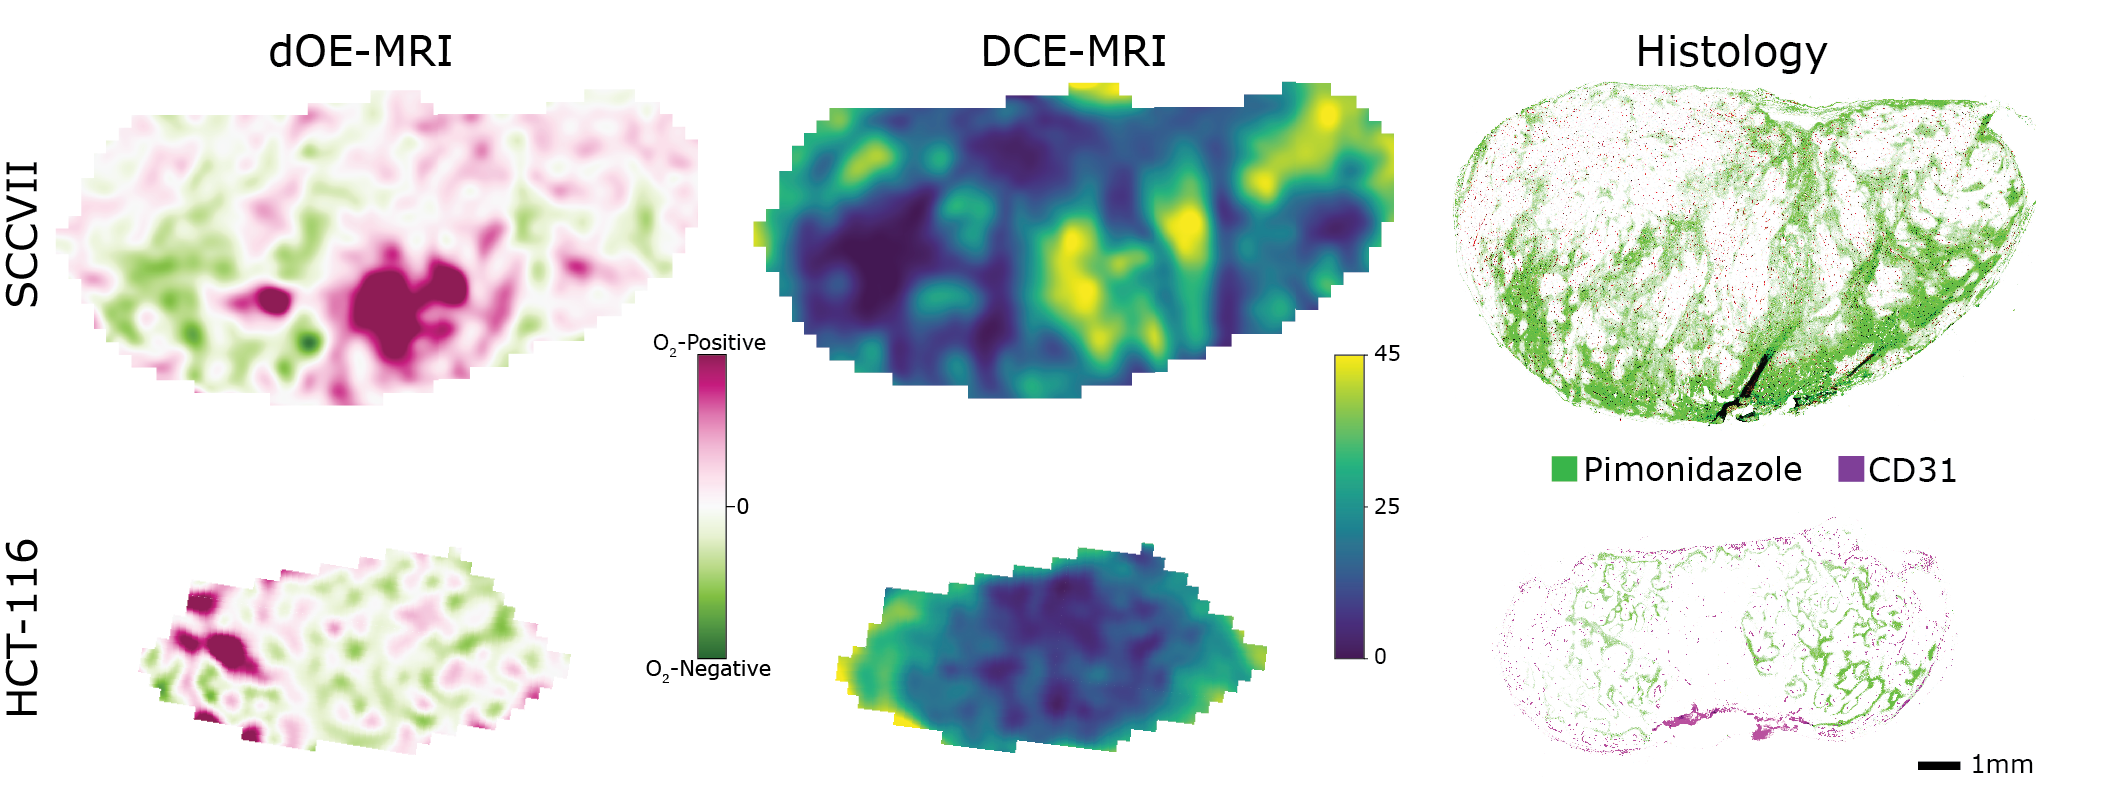
\includegraphics[width=\textwidth]{futurework/futurework-images/fig_perfusion.png} % requires the graphicx package
   \caption{\ac{dOE-MRI} maps and DCE-MRI IAUC$_{60}$maps and slice-matched histology sections of SCCVII and HCT-116 tumours. Large regions marked as purple in the \ac{dOE-MRI} maps are O$_2$-positive and also correspond to regions that have high IAUC$_{60}$ values (yellow). Green or O$_2$-negative regions from the \ac{dOE-MRI} map are often consistent with unperfused regions in the IAUC$_{60}$ (black), but there are regions of mismatch. Histology images stained with pimonidazole (green) and CD31 (purple) are shown for corresponding sections.
   \label{fig_perfusion}}
\end{figure}

\section{Adding T2* to the mix}

%%% from the grant
\todo{this is currently cribbed from the grant, it needs to be DRASTICALLY shortened, and edited for appropriateness, receptiveness, and overall style}
An alternate approach is to simultaneously acquire R1-weighted and R2*-weighted data to improve specificity of the technique[21]. R2* imaging would utilize the Blood Oxygen Level Dependent (BOLD) effect, which can measure shifts in hemoglobin saturation through changes in R2* and therefore assess tumour perfusion without the need for injectable contrast agents. Applying an oxygen challenge also shifts the haemoglobin saturation and, thus, the R2* signal. A postulated biophysical mechanisms is shown in Appendix Fig A2. The expected behaviour of a joint change in R1 and R2* in response to a gas challenge, and how this can be interpreted to reflect tumour oxygenation is based on data from last year?s work by Little et al.[21] and Waterton et al.[23]. The altered R2* provides a robust measure of areas with functioning vasculature. Subsequently, dOE-MRI maps can be masked using the ?R2* maps to exclude unperfused regions and enable improved SNR for R1-weighted signals, resulting in a completely endogenous technique to assess tumour oxygenation. OE-MRI T1-weighted signal more directly reflects oxygen amounts in plasma and tissues and is more applicable for measuring tumour oxygenation as it relates to radiotherapy.
Without sacrificing the information obtained from R1-weighted signal intensity in our current work, it is possible to extract both R1-weighted signal intensity and R2* simultaneously using a dynamic, multi-gradient echo in place of a dynamic FLASH sequence. We propose that our cycling gas challenge in combination with ICA improvement to R1-weighted OE-MR imaging may also be applicable to R2*, and we will test them in combination as an approach to improve the specificity of OE-MRI and therefore increase its capacity for clinical application. 
We propose to further develop dOE-MRI as a biomarker of the tumour microenvironment using simultaneous R1 and R2* imaging: vector-dOE-MRI. This proposal is a logical continuation of the OE-MRI efforts in the Reinsberg and Minchinton labs. The expected outcomes are an important part of a wider hypoxia-targeting effort. A previous grant application with Minchinton as nominated PI has been significantly simplified and re-focussed on the method-development aspect.

%% from approaches & methods

In achieving Objective 1 we will prove that (hypothesis 1) 	our current ICA approach to extract R1-dOE-MRI can be applied to oxygenation-induced changes to R2* from the multi-gradient echo.

In preliminary work we have established that a multi-gradient echo (MGE) sequence is ideal to extend our current R1w dOE-MRI technique [3] to also acquire dynamic R2* data: Initial echoes from an MGE sequence are  R1w and as the echo time increases, the images become more R2*W. The R1w-dOE-MRI map will be calculated from the signal
intensity of the first gradient echo image (minimal echo time TE=2.25 ms). The R2*- dOE-MRI map will be created by applying ICA to the mono-exponentially fitted multi-gradient echo data at each repetition. Fig 4 outlines our approach to obtain R1- and R2*-based dOE-MRI maps from a single multi-gradient echo sequence. Our current experience shows that while the temporal resolution of the multi-gradient echo technique is lower, the data quality of the R1w-dOE-MRI map is not compromised until subsampling exceeds six times the original temporal resolution when compared to that obtained with a FLASH sequence. Details on the impact of lower time resolution are in Appendix Fig A3.
To test our hypothesis we will conduct an imaging study that pits our established FLASH acquisition and ICA technique against the new approach of multi-gradient echoes in a panel of tumour xenograft models exhibiting varying patterns of hypoxia and perfusion. Initially, a Look-Locker sequence to measure a baseline R1 map will be acquired (TE/TR=3.0ms/10000ms, individual inversion time=157ms repeated in 25 frames, geometry matched to subsequent image sequences: matrix=128x80, FoV 3.84cmx2.40cm). Each scan will be for a 30 min O2 challenge. For the first 15 minutes, data will be acquired using the standard R1w-dOE-MRI sequence (TE/TR = 2.67 ms/66.7 ms, ?=40�, temporal resolution of 4.3 s with 210 repetitions for a total scan time of about 15 minutes). Then we will acquire images using the multi-gradient echo sequence (first TE=2.25ms with eleven additional echoes every 2.5ms, TR=35ms, ?=15�, 8 slices, matrix 28x64, temporal resolution=18s, 50 repetitions for total scan time of 15min). We expect no difference between the independently acquired R1-dOE-MRI maps (FLASH vs. MGE) beyond the variability that can be observed in the temporal fluctuation during the 15 minutes experiment. For this comparison of FLASH- and MGE-derived R1-dOE-MRI map, we will follow our stability studies that were part of our initial development of the FLASH-based OE-MRI[3].
The numerical data processing required for ICA will be carried out using a suite of in?house software we developed using the python machine learning library scikit?learn[24], specifically sklearn.decomposition.FastICA. Since ICA is a blind-source estimation and no input of an expected response functions is needed, one can take the successful extraction of a component that is temporally synchronized with the oxygen challenge as proof that tissue R2* is responding to the systemic administration of oxygen. While this provides a test for the hypothesis under Objective 1, physiological relevance will be addressed under Objective 3 using comparison with perfusion assessment and histological information.

\begin{figure}[htbp]
   \centering
   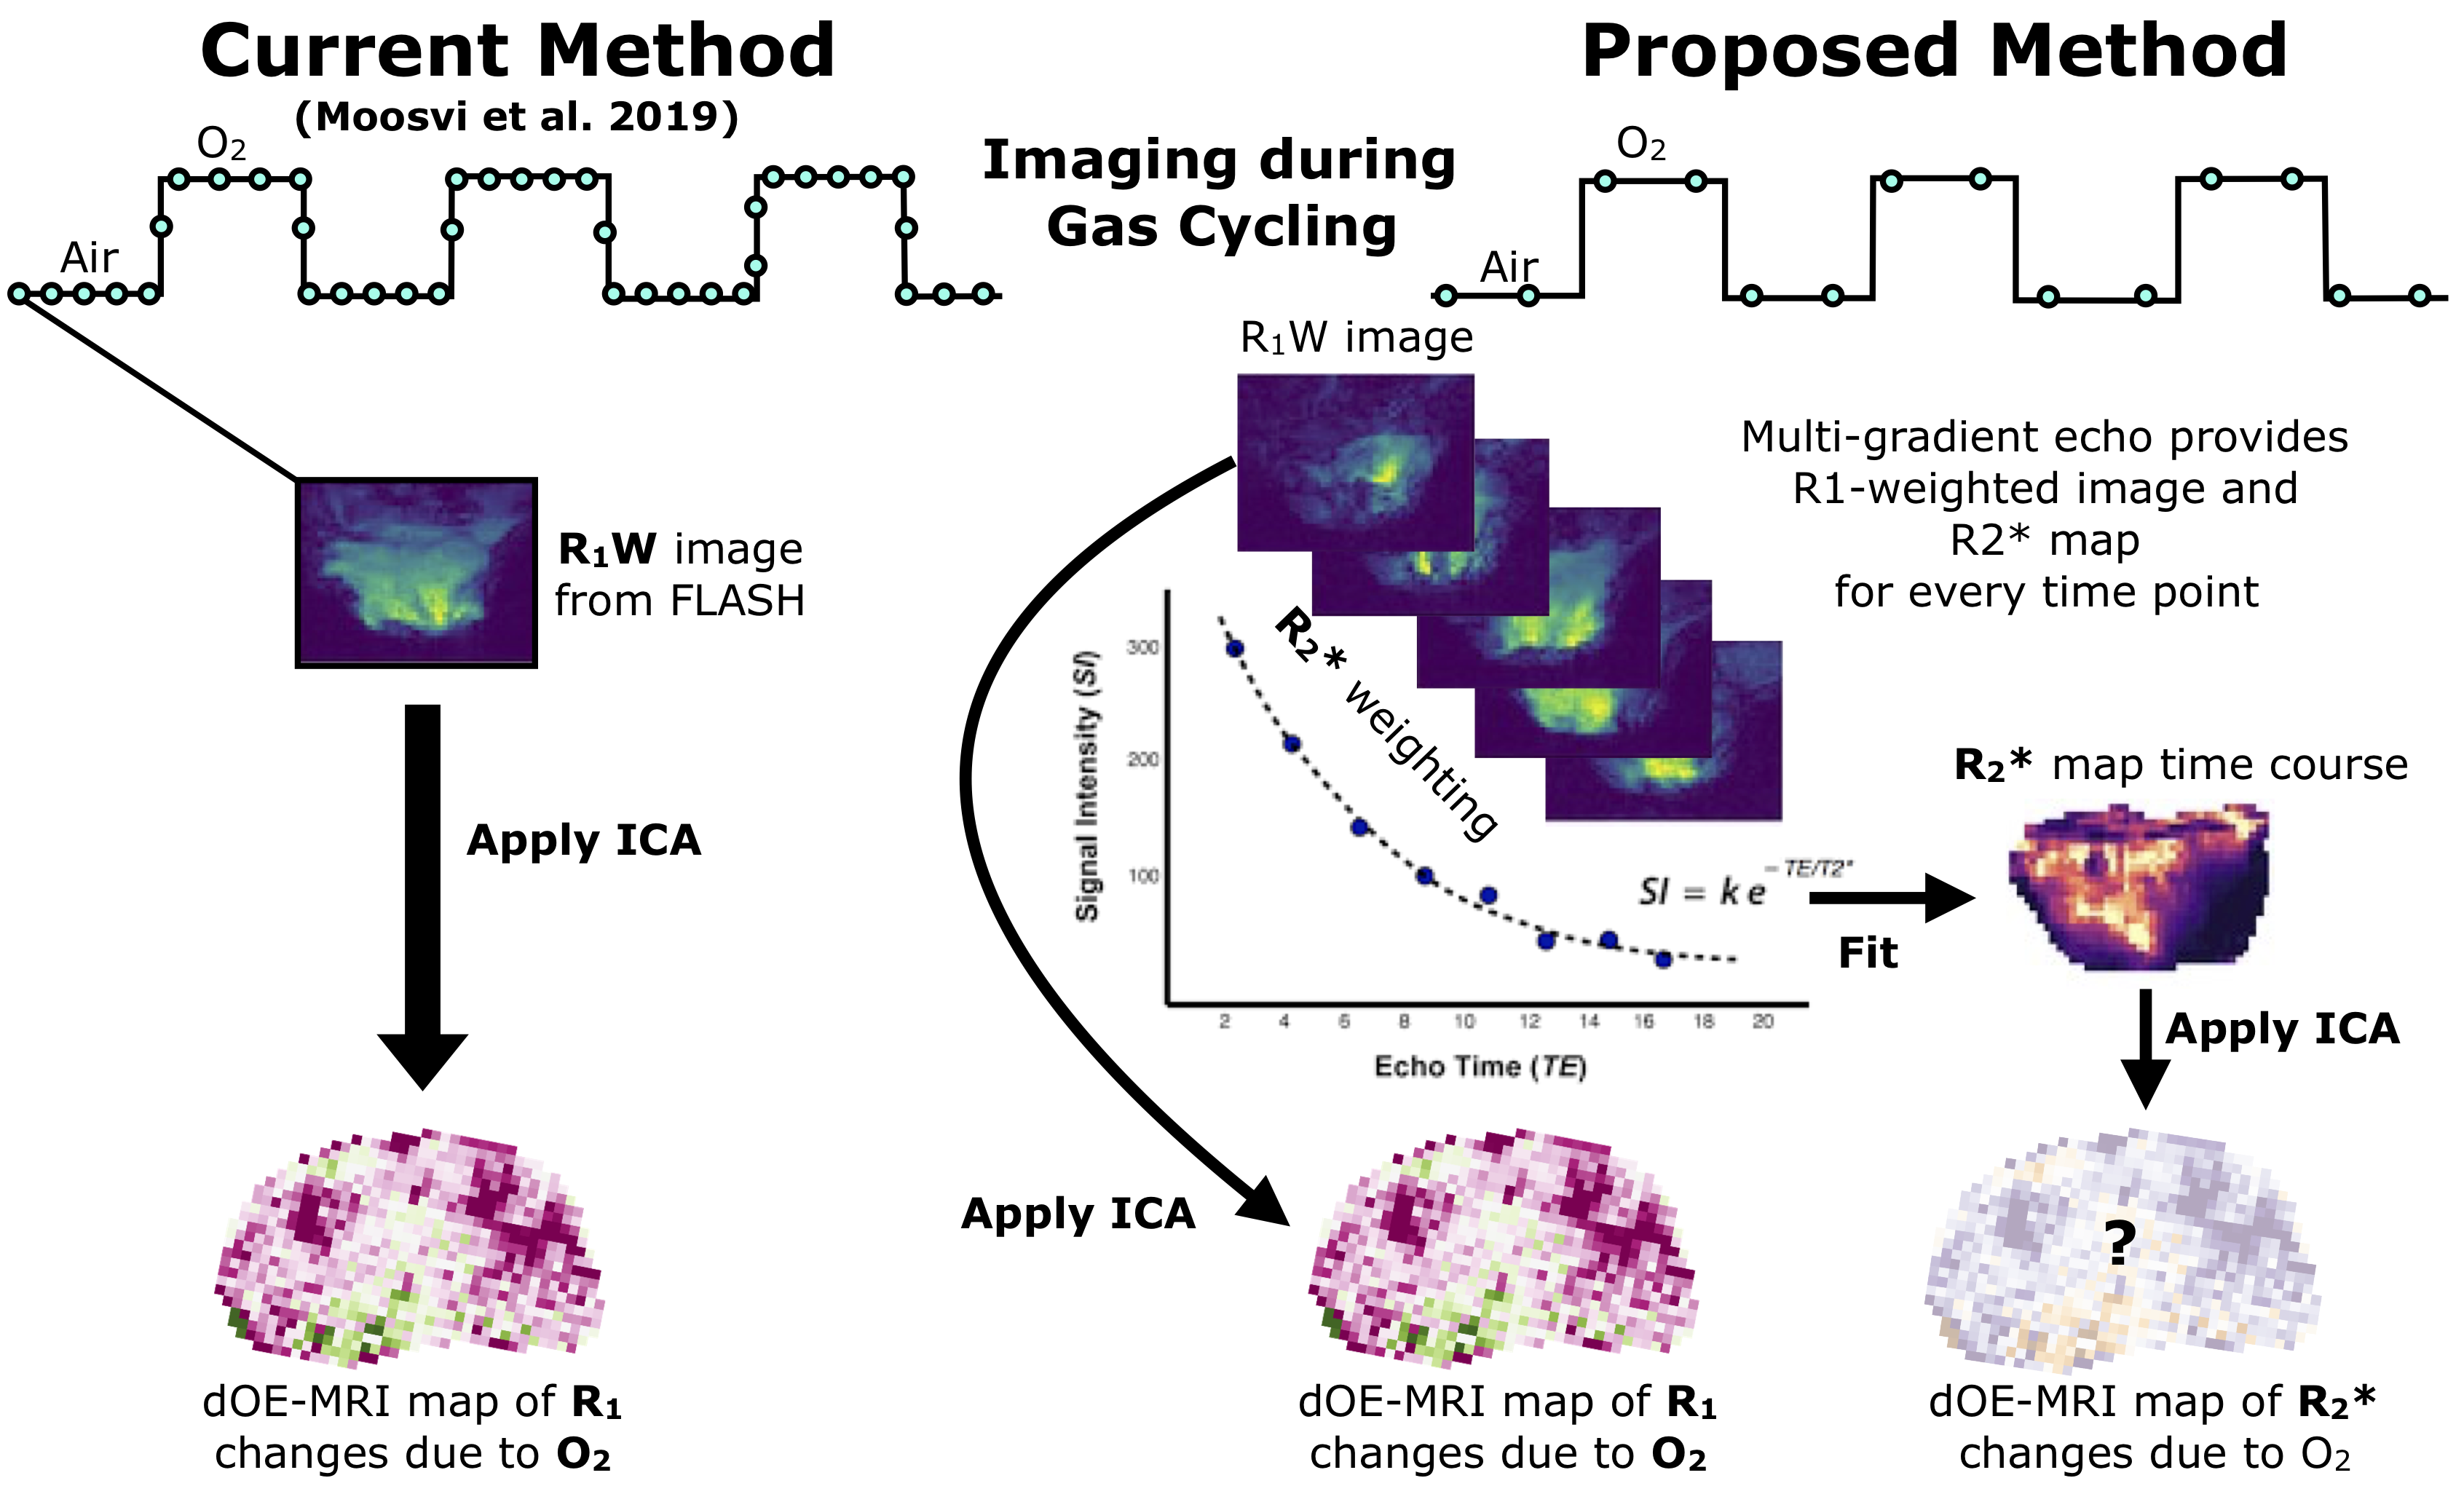
\includegraphics[width=\textwidth]{futurework/futurework-images/grantfig4_MGE_schematic.png} % requires the graphicx package
   \caption{Schematic of the current and proposed acquisition and analysis for \acs{dOE-MRI} with combined R$_1$ and R$_2$ imaging.
   \label{MGE_schematic}}
\end{figure}

\subsection{Independent Vector Analysis}

Our application of ICA to oxygen imaging increased the sensitivity of traditional oxygen-enhanced MRI such that one can investigate oxygen response on a pixel-wise basis rather than having to average R1w signal intensity or T1 changes over regions that are defined by perfusion selection[14,25]. We are planning to investigate whether this enormous gain in statistical power can be replicated by including a further MR parameter (R2*) in a vector-based blind-source estimation adapted from an analysis technique pioneered in fMRI. The problem solved by independent vector analysis (IVA) is that observations that are vector quantities (i.e. tuples consisting of one R1-weighted signal and one R2* from the exponential fit)  are explained by a mixture  of source vectors  [26?28]:

\begin{equation}
x_i = \sum_{j}^{L} a_{ij} \circ s_j
\end{equation}

where $\circ$ indicates an element-wise product. An algorithm suggested by Rafique et al. in 2016 solves the implementation problem and makes it available as FastIVA [29]. This algorithm can be readily implemented in our current analysis framework that makes use of sklearn?s FastICA. We will use FastIVA and analyse the multi-gradient echo data acquired under Objective 1. The independent components synchronized with the oxygen-challenge paradigm will be selected for the extraction of an oxygen-challenge related component map (recall that since this is a blind-source estimation we are not providing an expected response as prior to the analysis). This map will be tested for correlation with aligned tumour sections histologically analyzed for pimonidazole.

A current approach in the use of R1-based oxygen-enhanced MRI is to use a perfusion mask from a contrast-agent injection to exclude unperfused areas. The remaining perfused regions can then be classified into oxygen-refractory and oxygen-enhancing regions[14]. The use of a contrast agent injection complicates the imaging protocol and is being resisted by clinicians[17].
We will acquire MGE data using the sequence developed under Objective 1 and create masks from baseline R2* maps as well as R2*-dOE-MRI maps. Both masks will be applied to R1-dOE-MRI maps obtained through ICA of the first-echo time course from the same MGE data. To validate this technique, we will use the injectable macromolecular contrast agent \acs{HPG-GdF} for a dynamic-contrast enhanced scan. In our previously published methodology we calculated bolus arrival time (BAT), apparent permeability?surface area product (aPS), and fractional plasma volume (fPV) [30]. BAT is a robust marker of tumour vasculature in the use of HPG-GdF. This ?perfusion? parameter map will also be used to mask areas of perfusion within which to evaluate the R1-dOE-MRI map against the histologically evaluated hypoxia marker pimonidazole. When O?Connor et al. validated the R1w-dOE-MRI method, they correlated the oxy-refractory fraction in the perfused areas (regions with positive IAUC60) with pimonidazole staining[14]. We will compare the correlations from perfusion-masked OE-MRI maps (current standard) to the correlations obtained using masking with R2* baseline and R2*-dOE-MRI maps. We will further use the parameter map calculated using IVA (vector-dOE-MRI) as a third contender in the comparison with the current standard.

%%%% End from the grant






%\begin{figure}[htbp]
%   \centering
%   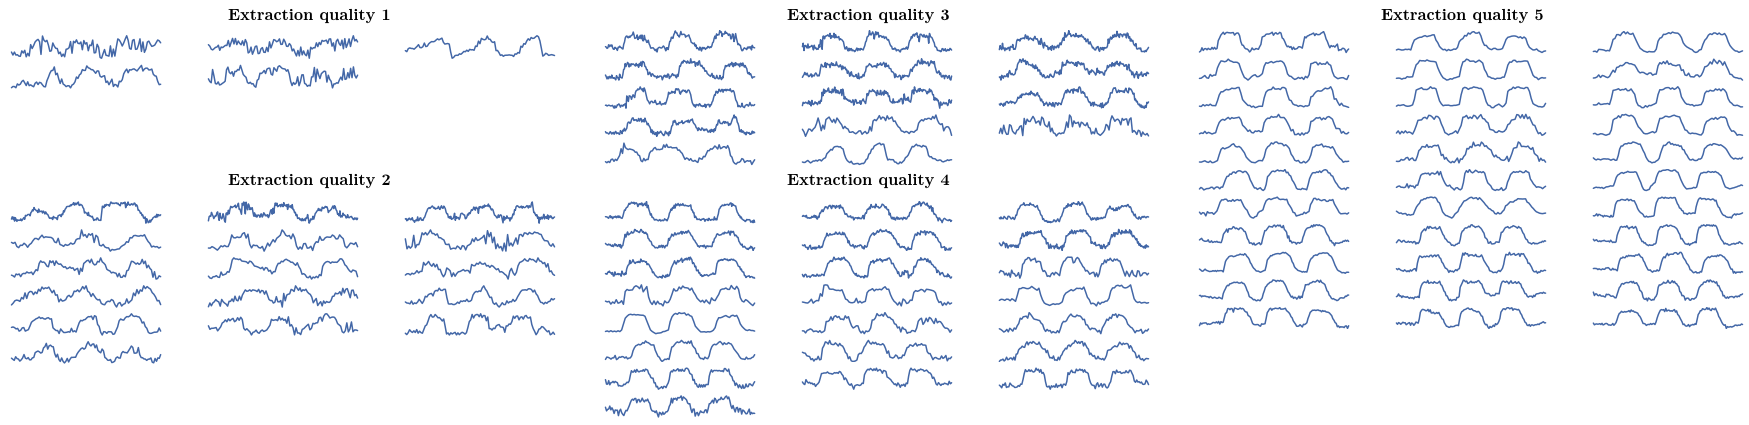
\includegraphics[width=\textwidth]{futurework/futurework-images/technical_ScoredExtractions.png} % requires the graphicx package
%   \caption{Each trace plot is the extracted ICA component corresponding to the oxygen response. The components are scored by the observer from a score of 1 to 5, with 1 barely corresponding to the oxygen challenge with a lot of noise and 5 corresponding extremely well to the oxygen challenge and very little noise. Note very few animals are in the lowest group, and many more are of extraction quality 4 and 5.}
%   \label{extractions}
%\end{figure}





\endinput